%------------------------------------------------------------------------
%Editar Diplomado
\hypertarget{cv:eliminarPaso}{\section{Eliminar Paso}} \label{sec:eliminarPaso}

	Esta funcionalidad le permitirá eliminar un paso innecesario o incorrecto. Para eliminar una paso es necesario que no se encuentre en referenciado en pasos de otros casos de uso o incluso en un otro paso del mismo caso de uso.

		\subsection{Procedimiento}

			%Pasos de procedimiento
			\begin{enumerate}
	
			\item Oprima el botón \IUBotonEliminar{} de un registro existente de la pantalla \ref{fig:GestionarPasos} ''Gestionar Pasos''.
	
			\item Se mostrará el mensaje \ref{fig:confirmaEliminaPaso} sobre la pantalla \ref{fig:GestionarPasos} ''Gestionar Pasos''.
			
			%Pantalla
			\begin{figure}[htbp!]
				\begin{center}
					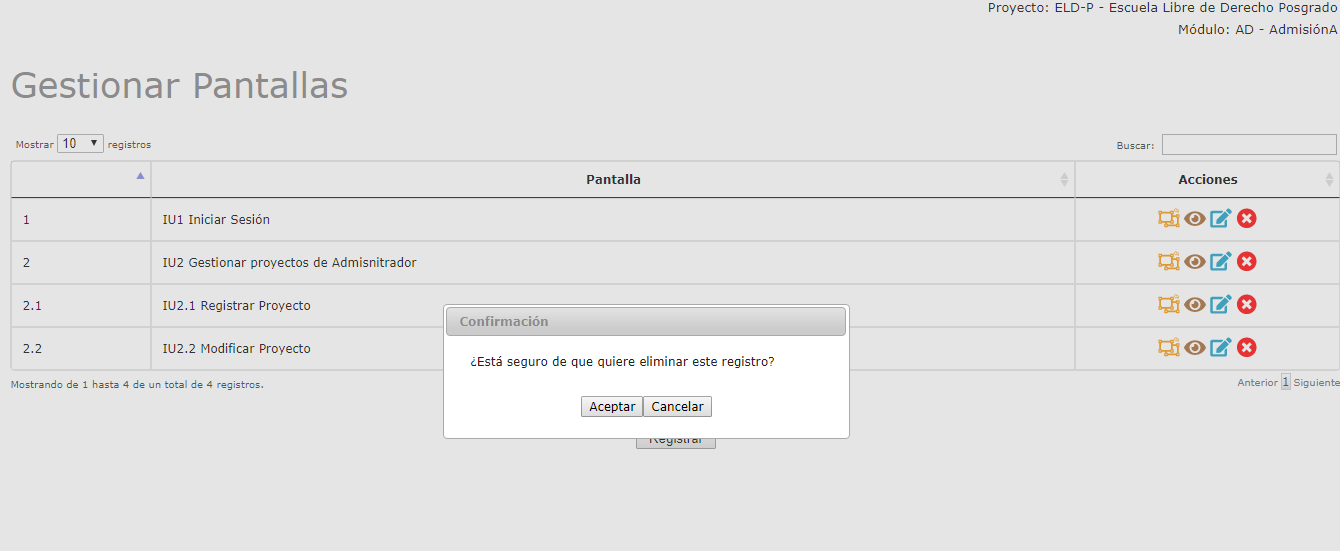
\includegraphics[scale=0.5]{roles/lider/casosUso/pantallas/IU11-3MSG10}
					\caption{MSG de Confirmación}
					\label{fig:confirmaEliminaPaso}
				\end{center}
			\end{figure}
						
			\item Oprima el botón \IUAceptar.
			
			\item Se mostrará el mensaje \ref{fig:pasoEliminado} en la pantalla \ref{fig:GestionarPasos} ''Gestionar Pasos''.
			
			\begin{figure}[htbp!]
				\begin{center}
					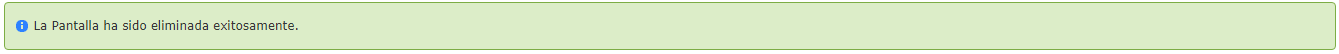
\includegraphics[scale=0.5]{roles/lider/pantallas/pantallas/IU11-3MSG1}
					\caption{MSG: Paso Eliminado}
					\label{fig:pasoEliminado}
				\end{center}
			\end{figure}
			\end{enumerate}